\documentclass[10pt,a4paper]{article}
\usepackage[margin=23mm]{geometry}
\usepackage[T1]{fontenc}
\usepackage{lmodern,microtype,amsmath,amssymb,booktabs,graphicx}
\usepackage[hidelinks]{hyperref}
\setlength{\parskip}{4pt}
\setlength{\parindent}{0pt}
\setlength{\emergencystretch}{2em}
\newcommand{\CoefZ}{1.918}
\newcommand{\MseZ}{1.911}
\newcommand{\EnergyZ}{2.031}
\newcommand{\OracleError}{1.73e-18}
\newcommand{\NegativePercent}{63.84}
\newcommand{\ClippedPercent}{43.60}
\newcommand{\ClippedRatio}{0.3710}

\title{QuantFlex: Sub-step Vibration Sensing and\newline Finite-sample Elastic-energy Bias}
\author{}
\date{Reproducible computational study, October 2026}
\begin{document}
\maketitle
\vspace{-2em}
\begin{abstract}
Can a sensor's quantization error be treated as independent noise when the
underlying vibration is smaller than one quantization step? An original synthetic
study combines exact oscillator response, uniform quantization, fixed-frequency
harmonic regression, and spring-energy estimation. Ordinary rounding can erase
the response at every sample, so longer records do not remove its bias.
Subtractive dither restores unbiased harmonic coefficients under explicit
independence and no-overload conditions, but adds a finite variance cost.
Across thirteen unclipped cases with 10,000 realizations each, coefficient means,
harmonic mean-square errors and corrected energy means agree with analytical
targets within respectively \CoefZ, \MseZ\ and \EnergyZ\ standard errors.
A deliberately saturated case violates those conditions. The results validate
the declared discrete experiment, not an instrument or a continuum model.
\end{abstract}

\section{Question, provenance and assumptions}
Uniform-quantization models in the locally available DTU MLSP sampling and
quantization material motivate the question above. The project explores their
limits for an idealized mechanical sensor; it does not reproduce course examples
or data. Subtractive dithering is established theory \cite{lipshitz}. The
contribution here is a reproducible implementation and a focused comparison of
coefficient error, nonlinear energy bias, and overload. Dither need not minimize
estimation error for every signal or noise regime \cite{rapp}.

Assume known forcing frequency, sample times and mechanical parameters, exact
dither subtraction, independent uniform dither, and an otherwise noiseless
sensor. Sampling is coherent and well above the forcing frequency. There is no
frequency identification, transient response, anti-alias filter, sensor drift,
material nonlinearity, or experimental calibration.

\section{Mechanical and measurement models}
The prescribed single-degree-of-freedom system obeys
\begin{equation}
 m\ddot u+c\dot u+ku=F\cos(\omega t),\qquad
 H=\frac{F}{k-m\omega^2+\mathrm{i}c\omega},\qquad
 u(t)=a\cos(\omega t)+b\sin(\omega t),
\end{equation}
where $a=\Re H$, $b=-\Im H$, $m,k,c>0$. This is the exact steady particular
solution. Set $\boldsymbol\beta=(0,a,b)^T$ and $X_i=(1,\cos\omega t_i,
\sin\omega t_i)$. The fitted offset is a nuisance term, not stored energy.
For a step $\Delta$, the midtread quantizer and subtractively dithered observation are
\begin{equation}
 Q_\Delta(x)=\Delta\lfloor x/\Delta+1/2\rfloor,\qquad
 y_i=Q_\Delta(u_i+d_i)-d_i,\quad
 d_i\overset{\mathrm{iid}}\sim\mathcal U(-\Delta/2,\Delta/2).
\end{equation}
Ties round upward. Without overload, the error $e_i=y_i-u_i$ is independent
uniform noise with variance $\sigma^2=\Delta^2/12$ \cite{lipshitz}.
The comparison uses $y_i=Q_\Delta(u_i)$ without dither. A separate overload
experiment clips integer codes to $[-1,1]$ before subtracting dither.
This symmetric three-level device is illustrative, not a bit-accurate commercial ADC.

\clearpage
\section{Numerical method and finite-sample predictions}
Reduced QR, $X=QR$, gives $L=R^{-1}Q^T$ and
\begin{equation}
 \widehat{\boldsymbol\beta}=L\boldsymbol y,\qquad
 C=\operatorname{Cov}(\widehat{\boldsymbol\beta})
 =\sigma^2LL^T=\sigma^2(X^TX)^{-1}.
 \label{eq:cov}
\end{equation}
No normal equations are solved in the implementation. Inputs are checked for
finiteness, shape, positive scales and full rank; designs with condition number
at least $10^8$ are rejected. Batches share one operator. Let $C_h$ denote the
cosine/sine block. For unbiased coefficients, the harmonic MSE is
$\mathbb E\|\widehat{\boldsymbol\beta}_h-\boldsymbol\beta_h\|^2
=\operatorname{tr} C_h$. For coherent integer periods with uniform samples,
$X^TX=\operatorname{diag}(N,N/2,N/2)$, so
\begin{equation}
 \operatorname{tr}C_h=\frac{\Delta^2}{3N}.
 \label{eq:mse}
\end{equation}
When $A=\sqrt{a^2+b^2}<\Delta/2$, ordinary rounding returns zero at every sample.
Its coefficient MSE is exactly $A^2$ regardless of record length. Dither has
smaller expected MSE in this regime only when $N>1/[3(A/\Delta)^2]$.
For $A/\Delta=0.05$, that threshold is $133\frac13$ samples; dither is therefore
expected to be worse at $N=40$ and better at $N=640$.

The target observable is cycle-average \emph{oscillatory} elastic energy,
\begin{equation}
 E=\frac{k}{4}(a^2+b^2),\qquad
 \widehat E=\frac{k}{4}(\widehat a^2+\widehat b^2),\qquad
 \widehat E_c=\widehat E-\frac{k}{4}\operatorname{tr}C_h.
 \label{eq:energy}
\end{equation}
Expanding the squares shows $\mathbb E\widehat E=E+(k/4)\operatorname{tr}C_h$;
thus $\widehat E_c$ is unbiased under the stated error model. Negative values are
retained: truncating at zero changes the expectation. This is an estimator of
nonnegative physical energy, not a claim that a spring stores negative energy.
The covariance and correction are deliberately not asserted for ordinary
rounding or saturated measurements.

\section{Implementation and reproducible experiments}
The Python package uses NumPy QR and vectorized matrix products; Matplotlib
produces the original figure. A native extension is unnecessary for these small
three-parameter fits. Public functions expose the quantizer, exact response,
harmonic model, covariance and energy. The quantizer returns an overload mask;
the caller is responsible for independent uniform dither. Validation checks
rounding ties, clipping, bad inputs, an independent real dynamic-equilibrium
system, direct cycle-energy integration, a least-squares oracle, and midpoint
integration of quantization-error moments. These distinguish algebra and
implementation checks from the Monte Carlo experiment.

Use $m=1$ kg, $c=0.4$ N\,s/m, $k=100$ N/m, $\omega=2\pi$ rad/s,
$\Delta=10^{-3}$ m and $t_i=i/40$ s for $i=0,\ldots,N-1$.
Choose $F=A|k-m\omega^2+\mathrm{i}c\omega|$ to prescribe
$A/\Delta\in\{0.05,0.2,0.8,2\}$, with $N\in\{40,160,640\}$.
Add a zero-amplitude case at $N=160$ and a clipped $A/\Delta=2$, $N=160$ case:
fourteen cases total. Each uses 10,000 independent dither records from NumPy's
default PCG64 generator, seeds $20261020+j$ in the listed amplitude-major order,
then zero and clipped cases. Coefficient-mean standard errors use the diagonal
of $C/10000$; energy and MSE means use empirical standard deviations divided
by $\sqrt{10000}$. These are Monte Carlo
standard errors, not guaranteed confidence intervals for a measured instrument.

\clearpage
\section{Measured results}
\begin{figure}[h!]
 \centering
 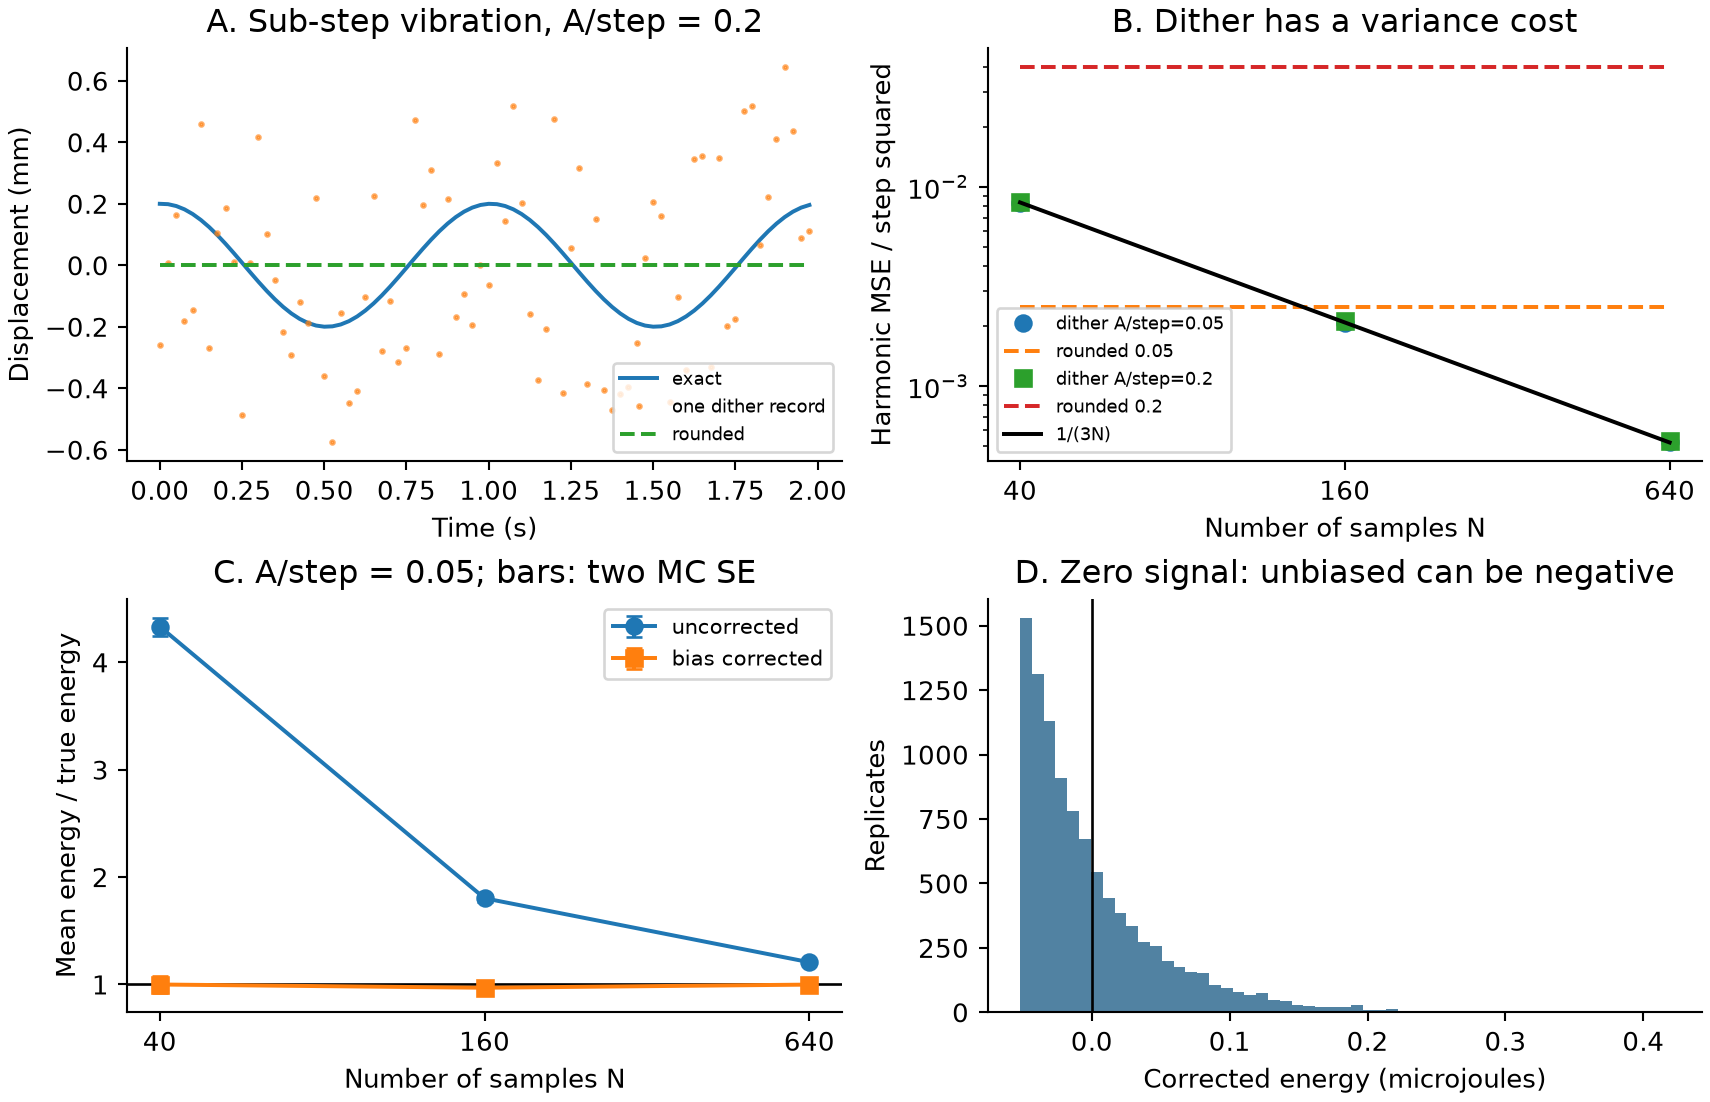
\includegraphics[width=\linewidth]{../results/study.png}
 \caption{Original outputs: (A) exact, rounded and one dithered record;
 (B) harmonic MSE and its finite-sample target; (C) energy means and twice their
 Monte Carlo standard errors; (D) corrected energy for zero true displacement.
 Curve comparisons are within the prescribed synthetic oscillator.}
 \label{fig:study}
\end{figure}
\begin{table}[h!]
\centering
\caption{Selected recorded cases. MSE columns are divided by $\Delta^2$;
 the last column is mean corrected energy divided by true energy.}
\begin{tabular}{rrrrrr}
\toprule
$A/\Delta$ & $N$ & Rounded MSE & Dither MSE & Theory MSE & $\overline E_c/E$\\
\midrule
0.05 & 40 & 0.00250 & 0.00827 & 0.00833 & 0.999 \\
0.05 & 640 & 0.00250 & 0.00052 & 0.00052 & 0.998 \\
0.20 & 40 & 0.04000 & 0.00833 & 0.00833 & 0.998 \\
0.20 & 640 & 0.04000 & 0.00053 & 0.00052 & 1.003 \\
\bottomrule
\end{tabular}

\label{tab:results}
\end{table}
The low-amplitude records confirm the predicted crossover: at $A/\Delta=0.05$,
dither increases harmonic MSE for 40 samples but decreases it for 640 samples
(Table~\ref{tab:results}). More samples cannot recover a signal whose ordinary
quantized record is identically zero. The full CSV includes the larger amplitudes,
which are not covered by the simple zero-output argument.

Over all thirteen unclipped cases, the largest absolute discrepancy is
\CoefZ\ standard errors for a coefficient mean, \MseZ\ for harmonic MSE,
and \EnergyZ\ for corrected energy. These finite-seed observations support
the analytic calculation; they do not prove a distributional theorem.
The QR estimates and independent least-squares oracle differ by at most
\texttt{\OracleError}\ m. The zero-signal corrected energy is negative in
\NegativePercent\% of records, consistent with retaining an unbiased quadratic
estimator rather than enforcing a physical constraint on each realization.

\clearpage
\section{Discussion, limits and conclusion}
The clipped experiment saturates \ClippedPercent\% of codes. Applying the
unclipped covariance correction anyway gives a mean energy ratio of
\ClippedRatio. This deliberate misuse demonstrates that subtraction of a
nominal noise variance cannot repair a biased nonlinear observation operator.
Checking an overload mask is essential; absence of observed overload alone does
not prove future no-overload behavior or independent dither.

Error and validation notions must remain separate. \emph{Discrete implementation error}
is assessed through the QR oracle, rounding rules, covariance identity and
independent equilibrium tests. \emph{Statistical error} is the finite-record
coefficient variance and finite-replicate uncertainty; dither trades deterministic
bias for this variance. \emph{Continuum error} is not measured: the continuous
steady oscillator is evaluated analytically, with no spatial mesh or time-stepping
approximation. Increasing $N$ extends the observation duration at fixed sampling
rate; it is not a continuum-convergence experiment. \emph{Physical validity}
requires separate evidence for actual stiffness, damping, forcing, sensor transfer
function and dither hardware. No such experimental evidence is supplied.

Exact frequency, steady response, noiseless analog measurements and exact dither
subtraction are strong assumptions. Correlated dither, subtraction mismatch,
colored sensor noise, unknown frequency or a nonuniform quantizer change the
covariance model. The code rejects gross numerical overflow and ill-conditioning
but does not certify metrology-grade floating-point accuracy. The energy estimate
excludes DC preload energy and has no positivity guarantee. No optimality,
universal benefit from dithering, hardware feasibility or runtime speedup is claimed.

Under its stated conditions, QuantFlex recovers the predicted covariance and
removes the finite-sample quadratic bias in an elastic-energy estimate. For
sub-step signals, record length determines whether this unbiased strategy has
lower coefficient MSE than complete suppression by rounding. Saturation can
invalidate both the uncertainty calculation and the correction. The repository
therefore makes the observation assumptions visible alongside the mechanics.

\section*{Reproduction and availability}
The repository contains original source, tests, recorded JSON/CSV values and
this manuscript: \url{https://github.com/racostacme-come/quantflex}.
Install Python 3.11 or newer, create a virtual environment, and execute
\texttt{python -m pip install -e ".[dev]"}.
Run \texttt{python -m pytest -q} and \texttt{python scripts/check\_results.py}.
The latter recomputes every recorded numerical value in a temporary directory;
\texttt{quantflex --output results} regenerates the study files.
Compile with \texttt{python scripts/build\_paper.py}, using pdfLaTeX or Tectonic.
The build rejects undefined references, overfull boxes and more than five pages,
and records SHA-256 hashes of inputs and PDF. CI rebuilds independently and
uploads page renders. The README documents installation, API use and limitations;
the MIT license covers this original implementation and manuscript.

\begin{thebibliography}{9}
\bibitem{lipshitz}
S.~P. Lipshitz, R.~A. Wannamaker, and J. Vanderkooy.
Quantization and dither: A theoretical survey.
\emph{Journal of the Audio Engineering Society}, 40(5):355--375, 1992.
\href{https://aes.org/publications/elibrary/elibrary-page/?id=7047}{Public bibliographic record}.
\bibitem{rapp}
J. Rapp, R.~M.~A. Dawson, and V.~K. Goyal.
Estimation from quantized Gaussian measurements: When and how to use dither.
2019. \href{https://arxiv.org/abs/1811.06856}{arXiv:1811.06856}.
\end{thebibliography}
\end{document}
